\begin{figure}[t]
\centering
\begin{subfigure}{70mm}
  \centering
    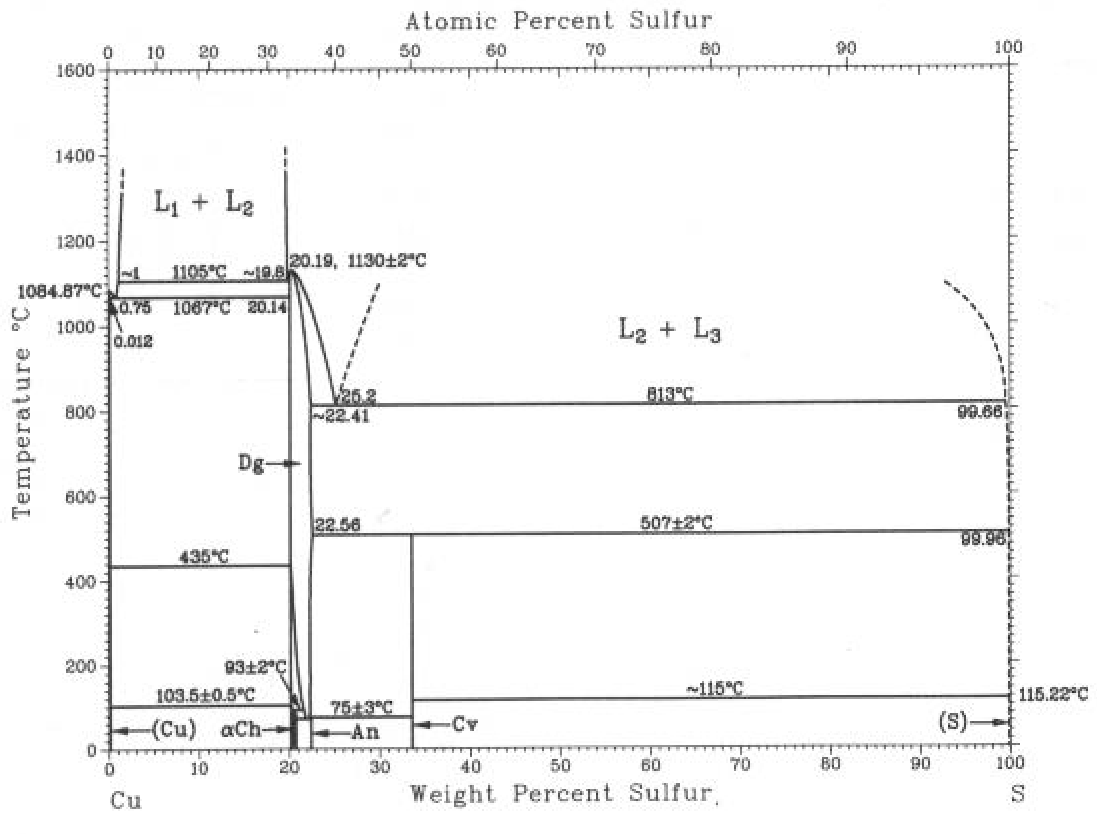
\includegraphics[width=70mm]{CuSAlloyDiag.png}
    \caption{Cu, S Binary Phase Diagram\citep{asm_international_asm_1992}}
    \label{fig:CuS}
\end{subfigure}%
\begin{subfigure}{70mm}
 \centering
    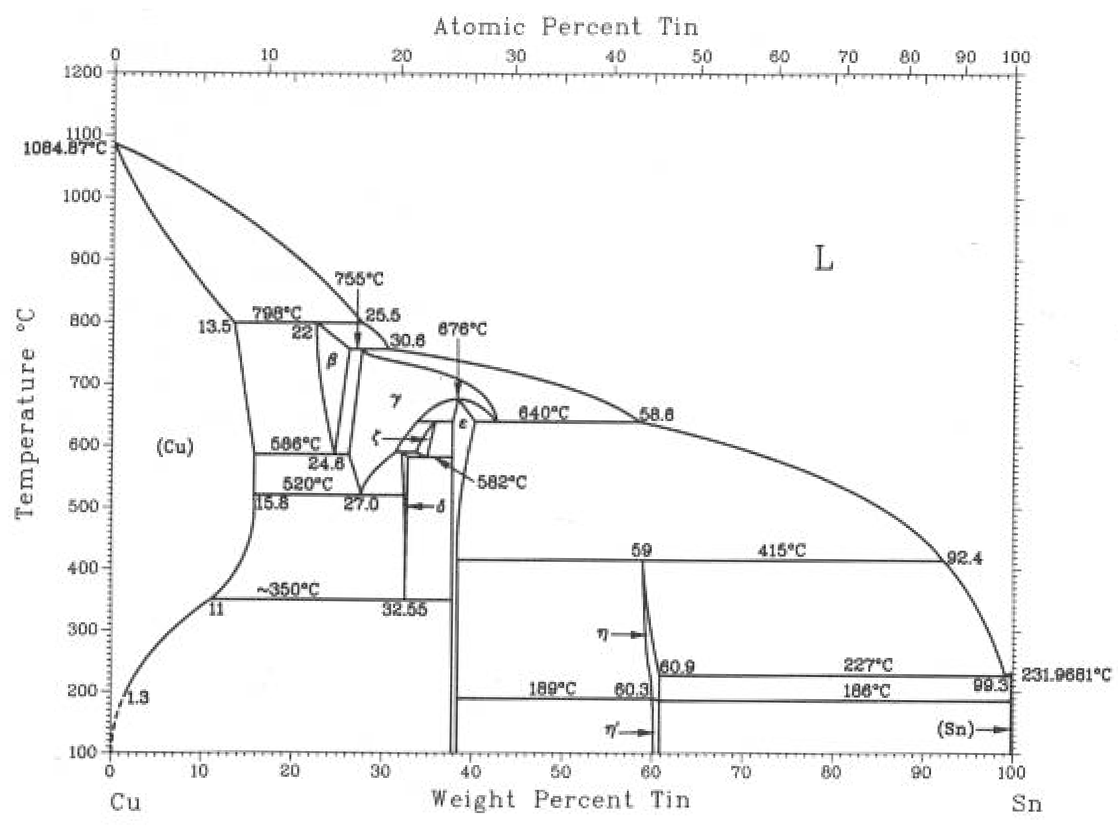
\includegraphics[width=70mm]{CuSnAlloyDiag.png}
    \caption{Cu, Sn Binary Phase Diagram\citep{asm_international_asm_1992}}
    \label{fig:CuSn}
\end{subfigure}
\begin{subfigure}{70mm}
 \centering
    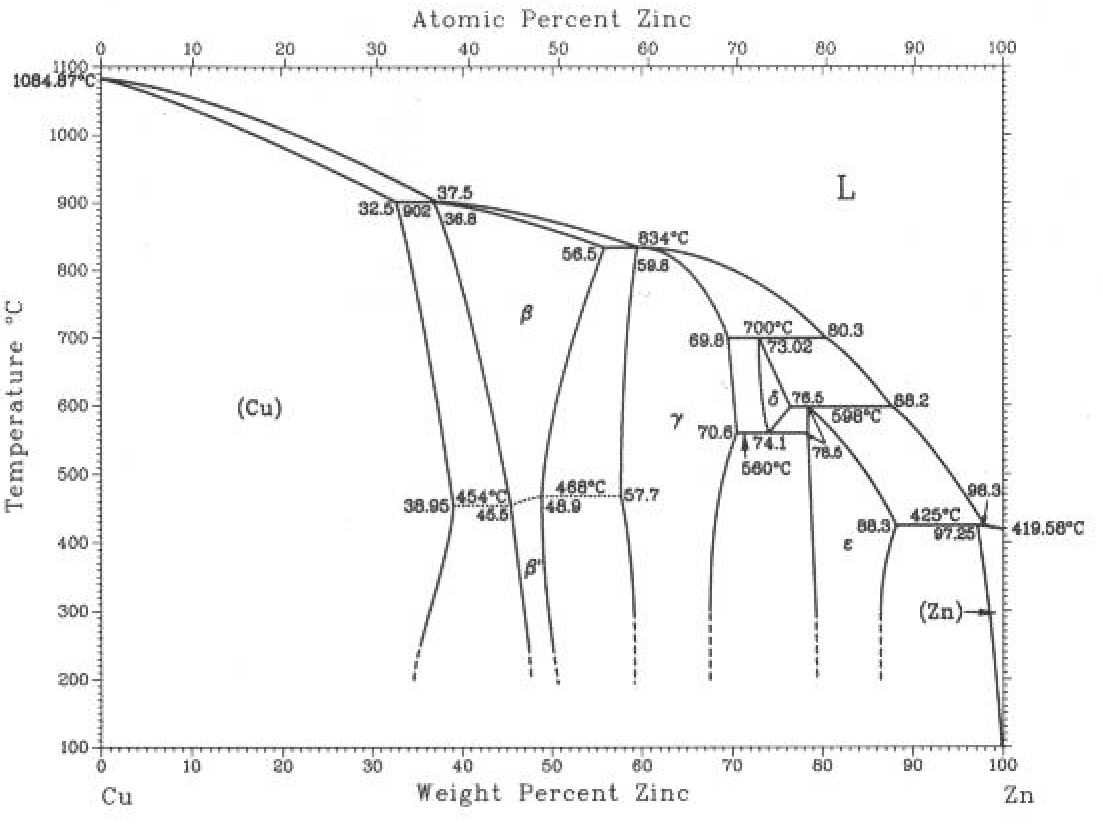
\includegraphics[width=70mm]{CuZnAlloyDiag.png}
    \caption{Cu, Zn Binary Phase Diagram\citep{asm_international_asm_1992}}
    \label{fig:CuZn}
\end{subfigure}
\begin{subfigure}{70mm}
 \centering
    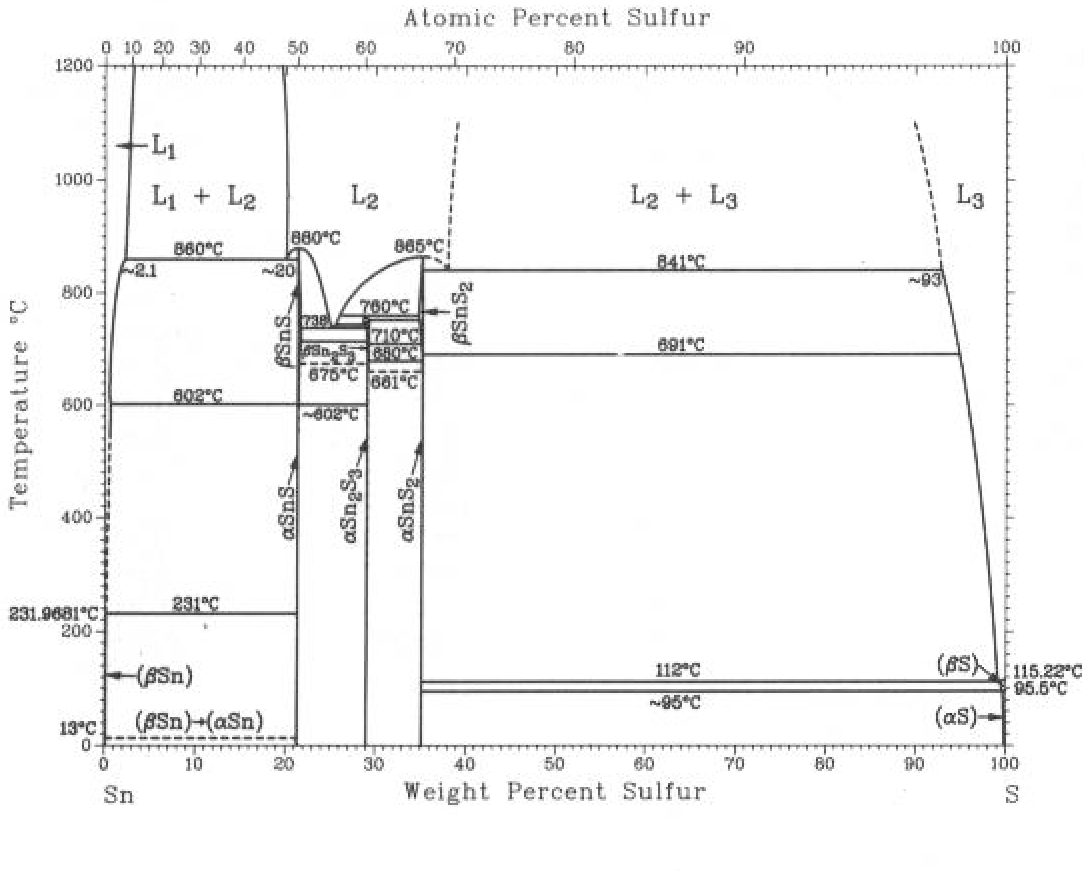
\includegraphics[width=70mm]{SnSAlloyDiag.png}
    \caption{Sn, S Binary Phase Diagram\citep{asm_international_asm_1992}}
    \label{fig:SnS}
\end{subfigure}
\begin{subfigure}{70mm}
 \centering
    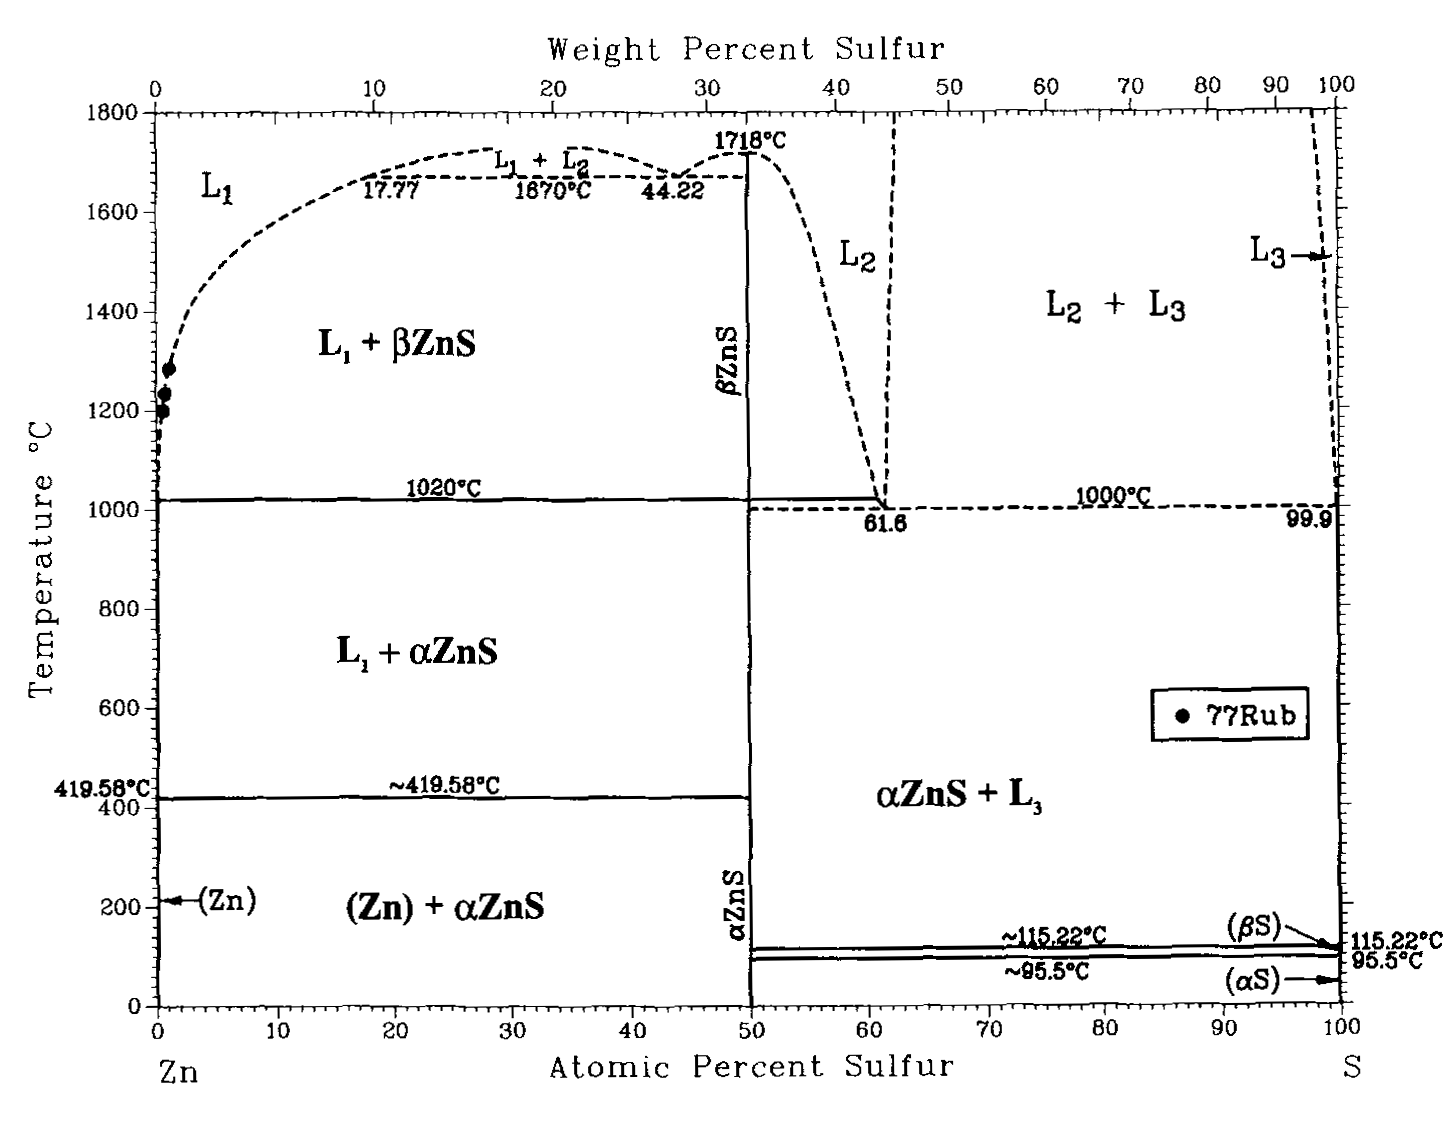
\includegraphics[width=70mm]{ZnSAlloyDiag.png}
    \caption{Zn, S Binary Phase Diagram\citep{sharma_s-zn_1996}}
    \label{fig:ZnS}
\end{subfigure}
\begin{subfigure}{70mm}
 \centering
    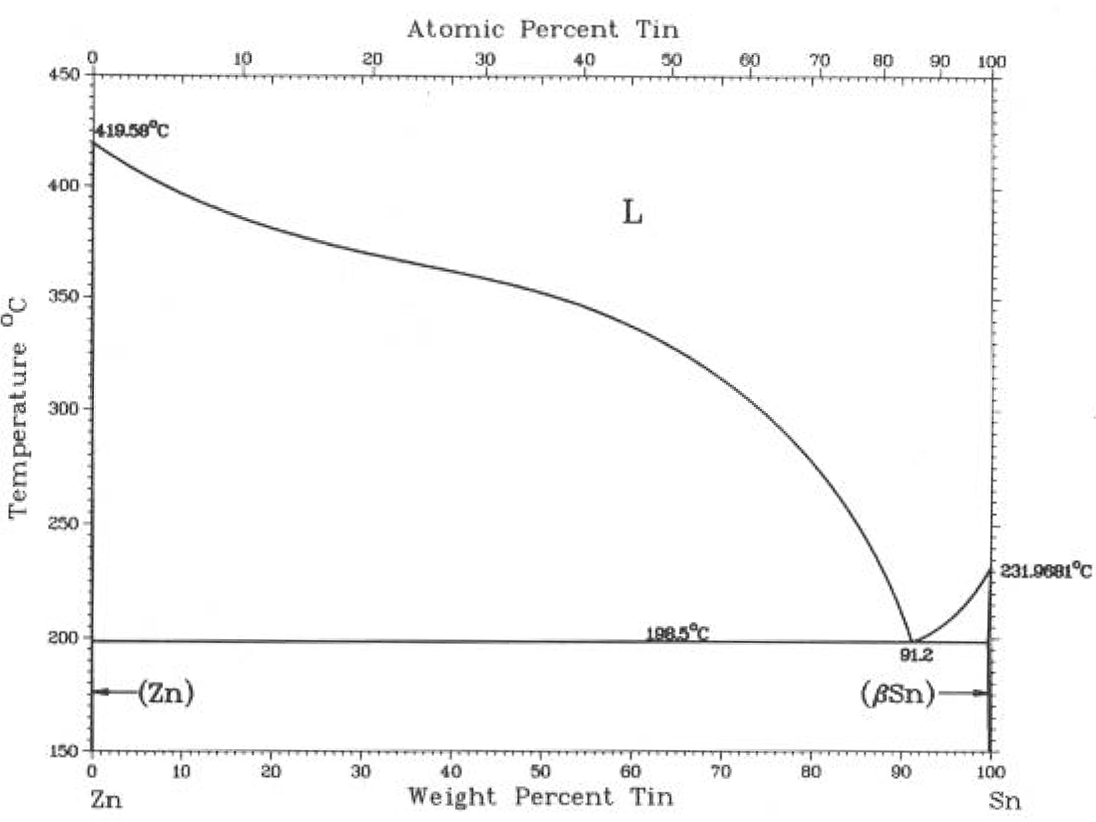
\includegraphics[width=70mm]{ZnSnAlloyDiag.png}
    \caption{Zn, Sn Binary Phase Diagram\citep{asm_international_asm_1992}}
    \label{fig:ZnSn}
\end{subfigure}
\caption{Binary Alloy Phase Diagrams Used in the calculation of the Ternary Phase Diagrams.}
\label{fig:BinaryAlloyPhaseDiagrams}
\end{figure}